\newcommand{\bmhBasicChapter}{BASIS-\\REGELN}
\newcommand{\bmhBasicHeadline}{Basis-Regeln}
\newcommand{\bmhBasicToc}{Basis-Regeln}
\newcommand{\bmhBasic}{%

	\dropping{W}enn ihr zum ersten Mal oder mit jungen Helden spielt, solltet ihr euch auf folgende Basis-Regeln beschränken. Zu den Experten-Regeln des folgenden Kapitels solltet ihr erst übergehen, wenn ihr etwas Übung habt.

	\bmhSection{Kreaturen}
		Jede Spielfigur stellt eine \keyword[Kreatur|basic]{Kreatur} dar.

		\example{Der Kämpfer, der Magier, ein Skelett -- all das sind Kreaturen.}

		\noindent
		\keyword[*]{Helden} sind auch Kreaturen, nur ganz besondere. Alle Regeln für Kreaturen gelten auch für Helden. Nur wenn explizit von \say{Helden} gesprochen wird, betrifft das nur diese.

	\bmhSection{Proben}
		Immer wieder musst du Attribute auf die \keyword[Probe|basic]{Probe} stellen. Dazu nimmst du so viele Würfel, wie die Zahl des Attributs beträgt, würfelst und zählst jene, die eine gerade Nummer aufweisen. So viele \keyword[Erfolg|basic]{Erfolge} hast du.

		\example{Hat dein Held Stärke~3 und würfelst du 2, 1 und 6, dann zählst du die 2 und 6 als zwei Erfolge.}

		\noindent
		Manchmal wird eine Probe leichter oder schwerer. Dadurch ändert sie die Zahl der Würfel, die du wirfst. Solltest du nach Abzügen auf 0 oder weniger Würfel kommen, darfst du nicht würfeln und hast automatisch null Erfolge.

		\example{Beträgt dein Geschick 2 und sollst du \say{GE+2 auf die Probe stellen}, würfelst du \bmhmath{2 + 2 = 4} Würfel, bei einer \say{GE Probe} \bmhmath{2 + 0 = 2} Würfel und bei einer \say{GE-1 Probe} nur \bmhmath{2 - 1 = 1} Würfel.}

	\bmhSection{Runden \& Züge}
		Das Spiel wird in \keyword[Runde|basic]{Runden} abgehalten. Die Spieler kommen, beginnend links vom SL, im Uhrzeigersinn an die Reihe. Sie führen dann für jede ihrer Kreaturen einen Zug aus. Ein Spieler muss den Zug einer Kreatur abschließen, eher er mit einer weiteren Kreatur zieht und muss mit allen seinen Kreaturen ziehen -- oder auf deren Zug verzichten -- ehe der nächste Spieler an die Reihe kommt. Als Letzter einer Runde zieht der SL, danach endet die Runde.

	\backgroundFooterFig[7.9cm]{%
		\begin{multicols}{2}\raggedbottom
			\color{white}\bmhBasicBoxExpose%
		\end{multicols}
	}

		Der \keyword[Zug|basic]{Zug} einer Kreatur besteht aus einer Folge von Aktionen. Ein Spieler hat dabei die Wahl, ob seine Kreatur~\ldots

		\bmhList{
			\item sich bewegt oder etwas benutzt, dann
			\item angreift oder sucht
		}

		{\centering\ldots~oder~\ldots}

		\bmhList{
			\item angreift oder sucht, dann
			\item sich bewegt oder etwas benutzt
		}

		{\centering\ldots~oder~\ldots}

		\bmhList{
			\item eine Fähigkeit einsetzt
		}

		{\centering\ldots~oder~\ldots}

		\bmhList{
			\item sich bewegt oder etwas benutzt, dann
			\item sich nochmals bewegt oder etwas benutzt, dann
			\item sich nochmals bewegt oder etwas benutzt.
		}

		\noindent
		Ein Spieler muss nicht alle Aktionen zu Beginn des Zuges ansagen, sondern kann den Ausgang einer Aktion abwarten, ehe er weitere Aktionen plant.

	\backgroundFooterFig[6.9cm]{%
		\begin{multicols}{2}\raggedbottom
			\color{white}\bmhBasicBoxDistance%
		\end{multicols}
	}

	\bmhSection{Aktionen}

		\noindent
		Dieser Abschnitt erklärt dir, was dein Held mit den \keyword[Aktion|basic]{Aktionen} machen kann.

		\bmhSubsection{Bewegen}
			Mit einer Bewegung darf deine Kreatur bis zu so viele Felder horizontal, vertikal oder diagonal weit gehen, wie ihr BEW-Wert beträgt. Dabei darf sie natürlich nicht durch geschlossene Türen oder Mauern gehen.

			Manche Felder werden durch Geröll, Treppen, Tische oder andere Hindernisse zu \keyword[Gelände!schwierig|basic]{schwierigem Gelände} und werden deshalb vom SL mit einem kleinen \say{x} am Spielplan markiert. Sie zu betreten kostet 2 BEW. Ein Feld, in dem eine andere Kreatur steht, gilt ebenso als schwieriges Gelände. Es zu durchschreiten ist allerdings nur mit ihrer Zustimmung erlaubt.

			Gelangst du während des Zuges neben ein unbekanntes Feld, kannst oder musst du den SL bitten, aufzudecken (siehe Kasten). Danach kannst du dich weiter bewegen oder deinen Zug gemäß den neuen Erkenntnissen anpassen.

			Deine Kreatur darf ihre Bewegung nicht auf einem Feld beenden, auf dem bereits eine andere steht.

		\bmhSubsection{Benutzen}
			Diese Aktion erlaubt dir, etwas aus deiner Ausrüstung oder deinem Umfeld zu \keyword{benutzen}. Du kannst damit:

			\bmhList{
				\item Dinge auf der Karte benutzen, wenn du direkt davor stehst, \zB~Türen öffnen/schließen oder Schalter betätigen
				\item einen Trank trinken, den du bei dir hast
				\item die Ausrüstung wechseln: Waffe, Rüstung, Schild oder Helm
				\item einer benachbarten Kreatur etwas übergeben
				\item etwas in deinem oder einem benachbarten Feld aufheben oder ablegen
			}

		\bmhSubsection{Angreifen}
			Nur wenn du Sicht zum Gegner hast und er in der Reichweite deiner Waffe steht, kannst du ihn angreifen. Egal ob Schwert oder Zauberstab, alle Waffen funktionieren nach folgendem Prinzip.

			Bestimme gemäß dem Kasten \say{Distanz} die Entfernung zu deinem Gegner. Nur wenn deine Waffe eine passende \keyword[Reichweite|basic]{Reichweite} (RW) hat, kannst du den Angriff durchführen.

			Ziehe nun eine Linie vom Mittelpunkt deines Feldes zum Mittelpunkt des Feldes des Gegners. Wird diese Linie durch eine Wand oder ein Hindernis blockiert, hast du \keyword[Sicht!keine|basic]{keine Sicht} und du darfst nicht angreifen. Streift die Linie bloß eine Ecke, oder durchquert sie ungehindert von Mauern nur die Felder anderer Kreaturen, hast du \keyword[Sicht!eingeschränkt|basic]{eingeschränkte Sicht}. Kannst du eine komplett ungehinderte Linie ziehen, hast du \keyword[Sicht!freie|basic]{freie Sicht}.

			Sieh jetzt bei deiner Waffe nach, was ihre \keyword[vs.|basic]{vs.-Angabe} ist. Das bestimmt, mit welchen Proben angegriffen und verteidigt wird.

			\example{Eine \say{ST vs. AB}-Waffe führst du mit deiner Stärke, dein Gegner verteidigt mit seiner Abwehr.}

			Mach nun eine Probe auf das Angriffs-Attribut. Hast du nur eingeschränkte Sicht, musst du mit einem Würfel weniger angreifen. Gib dann dem Gegner die Gelegenheit, eine Probe auf sein Verteidi\-gungs-Attribut zu machen. Für jeden Erfolg, den der Angriff mehr als die Verteidigung hat, verliert der Angegriffene einen \keyword[Lebenspunkte|basic]{Lebenspunkt}. Kreaturen, deren Lebenspunkte auf 0 fallen, sind \keyword[tot|basic]{tot} und werden vom Spielplan genommen. Bei Gegnern mit vielen Lebenspunkten führt ihr am Rand der Battlemap Buch, wie viele diese noch besitzen.

		\bmhSubsection{Fähigkeiten einsetzen}
			Jeder Held darf ein Mal pro Mission seine \keyword[Fähigkeit!einsetzen|basic]{besondere Fähigkeit einsetzen}. Dies nimmt einen ganzen Zug in Anspruch.

		\bmhSubsection{Suchen}
			Dein Held kann jederzeit nach Verborgenem \keyword[suchen|basic]{suchen}. Mach eine IN-Probe. Hast du mindestens einen Erfolg, muss dir der SL alle Schätze, Fallen oder Geheimnisse nennen, die sich auf deinem Feld und jenen der den acht direkt angrenzenden Feldern befinden, zu denen du Sicht hast. Schätze darfst du dir sofort behalten, kannst sie aber auch für andere Helden liegen lassen. Diese müssen sie dann nur mehr aufheben (siehe \say{Benutzen}).

			Suchen birgt aber das Risiko, dass eine \keyword[streunende Kreatur|basic]{streunende Kreatur}\index{Kreatur!streunend} auf dich aufmerksam wird. Sollte auf der Karte des SL in deinem Suchradius eine versteckte Kreatur eingezeichnet sein, wird diese aufgedeckt -- egal, ob die Suchen-Probe gelungen ist oder nicht. Im Missionstext ist angegeben, welche Kreatur das ist. Der SL stellt sie auf ein dir benachbartes Feld (oder ein möglichst nahes, sollten alle Felder belegt sein).

			Tipp: Ihr könnt erfolgreich durchsuchte Felder direkt am Spielplan markieren.
}

\newcommand{\bmhBasicGMHeadline}{Spielleiten}
\newcommand{\bmhBasicGMToc}{Spielleiten}
\newcommand{\bmhBasicGM}{%

	\bmhSection{Spielleiten}
	Als \keyword[Spielleiter|basic]{Spielleiter}\index{SL|basic} (SL) steuerst du keine Helden, sondern all die Kreaturen, die den Helden entgegen treten. Das ist weniger kompliziert und macht viel mehr Spaß, als es sich liest!

	Außerdem ist das kartographieren des Gemäuers deine wichtigste Tätigkeit. Achte bei jedem Schritt eines Helden darauf, ob du gemäß der Aufdecken-Regel neue Areale einzeichnen musst.

	Nicht alle Informationen der Mission sind für die Helden sofort sichtbar. Du kannst bedenkenlos alle Felder aufzeichnen, die kein Symbol in der unteren linken Ecke haben. Falls da aber doch ein Symbol ist, musst du aufpassen und den dazugehörigen Text lesen. Da diese Symbole für den SL bestimmt sind, werden sie nicht auf der Battlemap eingezeichnet.

	\bmhList{
		\item[\trap] Fallen werden am Plan nicht eingezeichnet.

		\item[\search] Diese Felder haben eine Besonderheit. Zeichne das Feld vollständig ein, aber lasse die Spieler nicht wissen, dass das Feld etwas verbirgt, das nicht im Vorlesetext erwähnt wurde. Wenn ein Held hier sucht, erfährt er die zusätzlichen Informationen aus dem Missionstext.

		\item[\monster] Hier lauern streunende Monster. Wenn ein Held hier erstmalig sucht -- egal ob erfolgreich oder erfolglos -- wird es aufgedeckt. Sollte das Feld bereits belegt sein, stelle die auftauchende Kreatur so nahe wie möglich auf den Spielplan.
	}

	\noindent
	Nachdem du das Spiel mit dem Vorlesen des Prologs und dem Aufzeichnen des Eingangsbereichs begonnen hast, kannst du dich erst einmal zurück lehnen und die Spieler handeln lassen.

	Sollten Monster auf dem Spielplan sein, darfst du mit diesen ziehen, wenn du an die Reihe kommst. Du darfst aber nur Monster ziehen, die bereits aufgedeckt wurden. Sie haben die selben Möglichkeiten wie die Helden, können aber nicht Suchen oder Aufdecken. Versuche, die Taktik jedes Monsters einzuhalten, die im Bestiarium (\refPage{lBestiary}) angegeben ist. Sie sind außerdem mit allen Fallen vertraut und können Fallenfelder durchschreiten, ohne diese auszulösen.

	\bmhSubsection{Fallen}
		Felder mit einem \trap-Symbol enthalten \keyword[Falle|basic]{Fallen}. Solange ihr mit den Basis-Regeln spielt, ignoriere die Beschreibung der Falle im Missionstext -- alle Fallen sind dann~\ldots

		\keyword[Falle!Pfeil-|basic]{Pfeilfallen}: Betritt ein Held ein Fallenfeld, ohne es vorher erfolgreich durchsucht zu haben, löst eine Falle aus: Eine Platte im Boden macht \say{Klick} und ein Pfeil kommt angeflogen. Der Held verliert 1~LP und seine Bewegung endet. Die Falle ist damit aber auch entschärft. Durchsucht ein Held erfolgreich ein Fallenfeld, wird die Falle entdeckt und automatisch entschärft.

	\bmhSubsection{Missionen}
		Du kannst mit den Basis-Regeln alle \keyword[Mission|basic]{Missionen} spielen, die für Helden der 1. Stufe geschrieben sind. Ab der 2. Stufe solltest du jedoch auf die Experten-Regeln umsteigen.
}

\newcommand{\bmhBasicBoxExpose}{%
	\keyword[aufdecken|basic]{AUFDECKEN}: Gelangt ein Held auf ein diagonal an Unbekanntem angrenzendes Feld, \emph{kann} sein Spieler den SL bitten, aufzudecken. Gelangt der Held auf ein Feld, das eine Seite mit Unbekanntem teilt, \emph{muss} der SL sofort aufdecken.

	\exampleInverted{Der Krieger (K) \emph{kann} aufdecken, der Schütze (S) \emph{muss}. Der Magier (M) ist nicht angrenzend und \emph{darf nicht} aufdecken.}

	Wird aufgedeckt, muss der SL den angrenzenden Gang oder Raum komplett einzeichnen, etwaige Monster auf den Spielplan stellen und weiteren Beschreibungstext vorlesen, falls das neue Areal einen hat.

	\medskip
	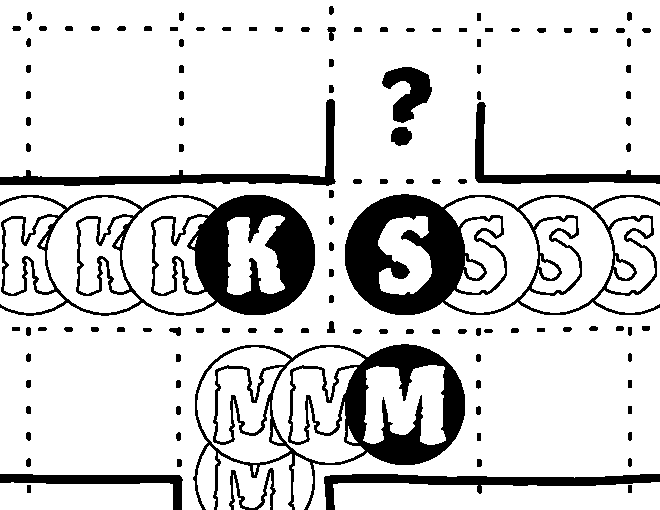
\includegraphics[width=\columnwidth]{\image{bmh/peek-basic.pdf}}
}

\newcommand{\bmhBasicBoxDistance}{%
	Um die \keyword[Distanz|basic]{DISTANZ} von einem Feld zu einem anderen zu ermitteln, zähle die Felder, die du minimal benötigst, um dieses auf direkter Linie horizontal, vertikal oder diagonal zu erreichen. Ignoriere dabei Hindernisse, Wände oder andere Figuren. Das Startfeld zählst du nicht mit, das Zielfeld schon.

	\medskip

	\exampleInverted{Die Goblins (G) sind vom Krieger (K) ein Feld entfernt, die Orks (O) zwei und das Skelett (S) vier.}

	\centering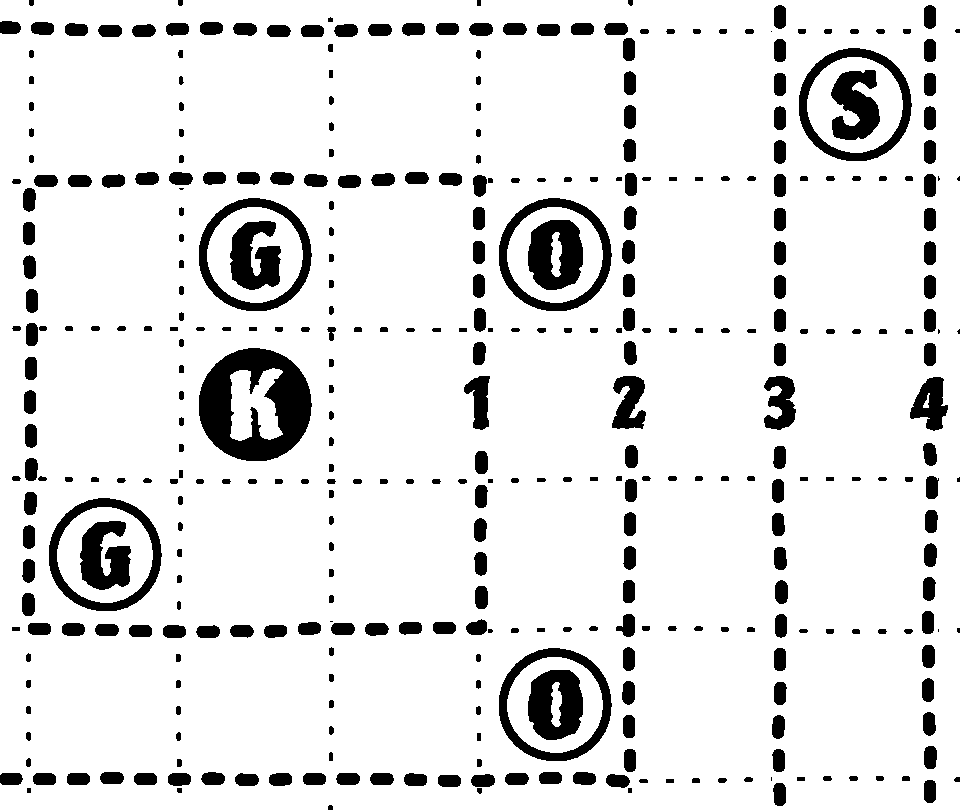
\includegraphics[width=\columnwidth]{\image{bmh/distance.pdf}}
}
